\chapter{Introduction}\label{chapter:introduction}

Magnetic Resonance Imaging (MRI) has found itself being used in an ever increasing number of applications. Uses range from imaging the spinal cord and heart to detecting brain activity (fMRI) and refinements to the technique have resulted in its use in fetal imaging increasing.

In many ways MRI is highly suited to fetal imaging; it has impressive contrast in soft tissue and no known harmful side effects. However, limitations in acquisition time causes movement to significantly impact the quality of the scan. A solution to this problem is to take a number of thickly sliced scans in a shorter time and use SVR (Slice-to-Volume Reconstruction) techniques to combine them.

These techniques work by registering (aligning) the slice stacks, which involves compensating for movement between slices, and then using super-resolution methods to construct a high resolution volume.

The quality of the reconstruction depends on the amount of motion in the original data. Areas with greater movement will be less well sampled which result in less data to use in the reconstruction, thus creating areas of high uncertainty.

From just looking at the reconstructed image it is not necessarily obvious where these high uncertainty areas are. Crucially when using these images for diagnostic purposes it very is important to be aware of this as if a diagnosis needs to be made based on a region of high uncertainty then this may indicate that further scanning is required.

The main aim of the project was to prototype visualizations to communicate this uncertainty to researchers and radiographers. This will allow them to both gauge the overall quality of the reconstruction and highlight any problem areas.

Two distinctive approaches have been prototyped and their effectiveness has been evaluated with a group of expert users. The first technique (section \ref{implementation:thresholding}) uses thresholding to find areas of the scan within a specific range of uncertainty; these areas can then be overlayed on the scan in 2D or displayed as a volume in 3D. The second technique projects the uncertainty to a surface. Two variations have been implemented, the first projects to a sphere (section \ref{implementation:sphere}) and the second projects to a representation of the object that has been scanned (section \ref{implementation:surface}).

The trade-offs between the two approaches have been studied to establish what works well and where future development should be focused. See section \ref{results:uncertainty_visualization}.

As well as visualizing the uncertainty, recent research\cite{uncertaintysvd} has shown that it is possible to use the uncertainty to guide the scanning process. The idea is that if we know, at the time of scanning, the areas of high uncertainty then we can then tailor the next scan position and direction to target these problem areas. A visualization designed to communicate this information has also been created. See section \ref{implementation:next_scan_plane}.

In addition to developing the visualizations a tool has been developed to begin to incorporate every stage of the reconstruction pipeline (see figure \ref{fig:tool_overview}) into one application. It allows the user to simulate scans, reconstruct an image and then utilize the visualizations.

\begin{figure}[h]
    \centering
  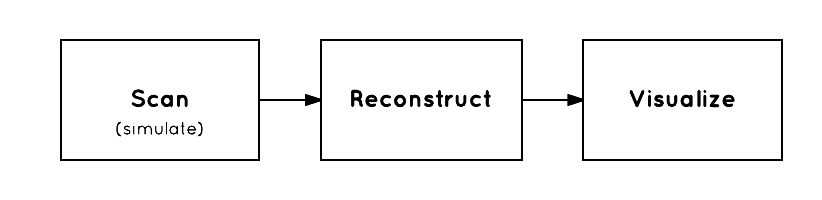
\includegraphics[width=0.8\textwidth]{images/tool_overview.png}
    \caption{Tool Overview}\label{fig:tool_overview}
\end{figure}

Simulating scans has been done previously to evaluate the performance of a reconstruction algorithm\cite{uncertaintysvd}. The idea is that we  assume a previous reconstruction is 'perfect', create lower resolution scans from it, run a reconstruction algorithm then compare the result to the original. This feature has been created to give a way for researchers to easily generate test data for reconstruction algorithms. See chapter \ref{implementation:scan_simulation}. The limitations of the current implementation are discussed in \ref{results:scan_simulation}.

One problem with the current fast GPU reconstruction implementation\cite{gpureconstruction} is that it is a command line application and the performance is heavily dependant on parameters being tweaked. To make the reconstructions easier to perform the reconstruction has been built into the tool. Additionally an enhancement to the reconstruction process has been trialled. One way to guide the reconstruction is by marking each slice stack with a set of landmarks (e.g. Left Eye, Right Eye, etc.); this helps the registration step align each of the stacks. A prototype to allow these landmarks to be marked on each slice stack before reconstruction has been created. See section \ref{implementation:reconstruction}. The researcher response to this feature is discussed in \ref{results:reconstruction}.